% Documents settings
\documentclass[twoside, openany]{report}

% Loading configs
% Defining some custom commands here...

% Custom variables
\def\SimWidth{\textwidth}
\def\SchematicWidth{0.7\textwidth}
\def\SmallSchematicWidth{0.24\textwidth}

% Standard paths
\def\Images{images}
\def\Config{config}
\def\Schematics{data/circuitikz}
\def\Drawings{data/tikz}
\def\Timings{data/timings}
\def\Tables{data/tables}
\def\Pdf{data/pdf}
\def\Code{data/code/Opale/application/src}
\def\Conf{data/code/Opale}
\def\DeviceTree{data/code/Opale/boards/topaze/DTSI}
\def\Src{chapters}

% Tikz timings
\usepackage{xparse} % NewDocumentCommand, IfValueTF, IFBooleanTF

% Reference a bus.
%
% Usage:
%
%     \busref[3::0]{C/BE}    ->   C/BE[3::0]
%     \busref*{AD}           ->   AD#
%     \busref*[3::0]{C/BE}   ->   C/BE[3::0]#
%
\NewDocumentCommand{\busref}{som}{\texttt{%
        #3%
        \IfValueTF{#2}{[#2]}{}%
        \IfBooleanTF{#1}{\#}{}%
    }}

% packages
\usepackage{float}
\usepackage{graphicx}
\usepackage{fancyhdr}
\usepackage{subfig}
\usepackage{caption}
% \usepackage[french]{babel}
\usepackage[T1]{fontenc}
\usepackage{hyperref}
\usepackage{minted}
\usepackage{amsmath}
\usemintedstyle{xcode}
\usepackage{placeins}
\usepackage{siunitx}
\usepackage{circuitikz}
\usepackage{pgfplots}


\hypersetup{
    colorlinks,
    citecolor=black,
    filecolor=black,
    linkcolor=black,
    urlcolor=black
}

\usepackage[	a4paper,
				top=25mm,	
				bottom=15mm,
				left=15mm,
				right=15mm,
				head=20mm,
				headsep=5mm]{geometry}
\usepackage[	style=ddmmyyyy,
				yearmonthsep={.},
				monthdaysep={.}]{datetime2}

\usepackage{tikz}

% Custom variables
\def\SimWidth{18cm}
\def\SchematicWidth{12cm}


% use the header and footer 
\pagestyle{fancy}

% Document informations
\author{Heywang Léonard - Charles Paolo}													
\title{Rapport de TP de Traitement du Signal}													
\date{\DTMtoday}


% Document informations
\author{Heywang Léonard, Brandstaedt Arthur}													
\title{Project report : Design of a control system for a small scale rocket}													
\date{\DTMtoday}

% Loading bibtex file
\addbibresource{quote.bib}

% Document
\begin{document}

% Setting font size
\fontsize{9}{10.5}\selectfont\blindtext

% Number pages in roman for the introduction (i, ii, iii)
\pagenumbering{roman}

\begin{titlepage}
	\raggedright
	\textbf{Heywang Léonard}	\\
    \textbf{Brandstaedt Arthur}  \\
	Students on the University of Strasbourg, Physics and Engineering departement\\
	1st year of Master in Electronics systems and Microelectronics (SEME))

	\raggedleft
	% Entreprise ...													
	% Addresse
	% Contact	

	\centering
	\vspace{3cm}

	\huge
	\textbf{Projet report : Design of a control system for a small scale rocket}\\
	Semester 1 and 2\\
    \vspace{0.5cm}
	\includegraphics[width=8cm]{images/logo.eps}

	\raggedright
	\normalsize
	\vspace{3cm}
	\textbf{Within the framework of the Master SEME :}\\
	Applied Physics and Engineering, \\
	Electronics systems and Microelectronics

	\vspace{1.5cm}
	\textbf{School year} 2024-2025

	\vspace{1.5cm}
	\textbf{Faculty of Physics and Engineering}\\
	3-5 Rue de l'Université, 67000 Strasbourg\\
	+33 3 68 85 07 30

	\vspace{1 cm}
	\centering
	\begin{figure}[!ht]%
		\centering
		\subfloat{{\includegraphics[width=5cm]{images/logo.eps} }}%
		\qquad
		\subfloat{{\includegraphics[width=5cm]{images/unistra.eps} }}%		
	\end{figure}
\end{titlepage}

% Header and footer definition
\fancyhead{}
\fancyhead[LE, RO]{Project report : Design of a control system for a small scale rocket}
\fancyhead[RE, LO]{
	\includegraphics[width=3cm]{images/logo.eps}
}

\fancyfoot{}
\fancyfoot[CE, CO]{\thepage}
\fancyfoot[RE, LO]{\DTMtoday}
\fancyfoot[LE, RO]{Heywang Léonard - Brandstaedt Arthur}


\tableofcontents
\listoffigures
\listoftables

\newpage
\chapter*{Introduction}
\addcontentsline{toc}{chapter}{Introduction}
\paragraph{}
This document cover the Opale project, which took place in the context inside the Master SEME
on the univeristy of Strasbourg.

\paragraph{}
This project was started on the first semester, by november 2024. The goal was to develop a
small scale rocket that modelize the behavior of real ones. This model include the usage
of powder engines, as well as come control electronics embedded into the rocket.

\paragraph{}
For all along this report, we're going to describe all the reflexions, studies, and conception.
Since we're Electronics Engineering students, we'll focus more on the electronics and sofware aspects,
but the mechanical part will also quicly be explained.
The goal with the control electronics is to ensure the rocket will follow a defined trajectory, as
well as storing into an EEPROM some measurements for an after fly interpretation.

The rocket can be modelled as a complex system, composed with multiples blocks :

\begin{itemize}[noitemsep]
    \item   Sensors (positionning, temperature...)
    \item   Outputs (Servos engines control, engine starter...)
    \item   Controller (MCU + Memory)
    \item   Power supplies
\end{itemize}

\paragraph{}
This report will be splitted in multiples parts, that are not ordered in a chronological order, but
more in a logic way.

\paragraph{}
In the first chapter, we're going to explain how we choosed main hardware elements, such as the controller,
the servo engines or the inertial measurement unit. Theses are device where a wide range of choices are possible !

In a second part, we'll focus on the caracterisation of some elements, to understand precisely how they respond to
any input signals. This is an important step if we want to develop a precise controller for them !

For a third chapter, we're going to detail the whole procedure of the electronic design. This start from the schematic,
and end up with a whole printed circuit board, ready to be manufactured.

For the next part, we'll see how we designed the controller of the rocket, the algorithm that compute the command to apply
to the wings to ensure a proper trajectory.

And, to finish the main section, a final part will be dedicated for the whole software we wrote, that handle the control as
well as some other task on the rocket.

After the conclusion, in annexes there will be some more details. This include a mechanical overview of the rocket, as well as
the process of soldering the board or some precisions about the software we developped.


\chapter*{System block diagram}
\addcontentsline{toc}{chapter}{System block diagram}
To ensure the reader will understand the following chapters, we drawned a 
block diagram, that summarize most of the important stuff on the project.

\begin{figure}[!hbt]
    \centering
    \resizebox{\SchematicWidth}{!}{%
        \begin{circuitikz}
            \tikzstyle{every node}=[font=\normalsize]
            \draw [ fill={rgb,255:red,195; green,232; blue,235} ] (8.75,14.75) rectangle  node {\LARGE MCU + Memory} (17.5,1);
            \draw [ fill={rgb,255:red,233; green,235; blue,199} ] (2.5,14.75) rectangle  node {\normalsize Sensors } (6.25,8.5);
            \draw [ fill={rgb,255:red,162; green,199; blue,179} ] (2.5,7.25) rectangle  node {\normalsize Users inputs} (6.25,1);
            \draw [ fill={rgb,255:red,236; green,195; blue,195} ] (8.75,19.75) rectangle  node {\normalsize Power supplies + Power managements IC (PMIC)} (17.5,17.25);
            \draw [ fill={rgb,255:red,218; green,187; blue,217} ] (20,14.75) rectangle  node {\normalsize Actuators} (23.75,11);
            \draw [ fill={rgb,255:red,158; green,148; blue,213} ] (20,9.75) rectangle  node {\normalsize USB Debug port} (23.75,6);
            \draw [ fill={rgb,255:red,158; green,148; blue,213} ] (20,4.75) rectangle  node {\normalsize User outputs} (23.75,1);
            \draw [->, >=Stealth] (6.25,4.75) -- (8.75,4.75);
            \draw [->, >=Stealth] (6.25,11) -- (8.75,11);
            \draw [->, >=Stealth] (17.5,12.25) -- (20,12.25);
            \draw [->, >=Stealth] (17.5,8) -- (20.25,8);
            \draw [->, >=Stealth] (17.5,3.5) -- (20,3.5);
            \draw [->, >=Stealth] (13,17.25) -- (13,14.75);
        \end{circuitikz}
    }%
    \caption{System block diagram}
    \label{fig:functionnel}
\end{figure}
\newpage

% Set page number in plain numbers (1, 2, 3...)
\pagenumbering{arabic}

\chapter{Component selection}
When starting the project, one of the first points was to choose components. But, 
why this one ? And not the other ? Let's dig into the hardware choices we made here !

\input{\Tables/list_servo.tex}
\begin{table}[!hbt]
    \centering
    \begin{tabular}{| c || c | c |}
        \hline
        Reference & Manufacturer         & Core specifications                              \\
        \hline
        \hline
        nRF5340   & Nordic Semiconductor & ARM Cortex M33 @128 MHz + ARM Cortex M33 @64 MHz \\
        STM32H5   & STMicroElectronics   & ARM Cortex M33 @250 MHz                          \\
        STM32F4   & STMicroElectronics   & ARM Cortex M4 @84 MHz                            \\
        ATSAMD51  & Microchip            & ARM Cortex M4F @120 MHz                          \\
        \hline
    \end{tabular}
    \caption{List of considered MCUs for the project}
    \label{tab:mcu_list}
\end{table}
\FloatBarrier

\chapter{Caracterisation and measures of actuators}
First, let's talk about the caracterisation of the engines :

First, we need to measure precisely how the engines respond to any arbitrary input, to design they're own control loop.
To measure the servo response, we proceeded in two times : A first session, with some electronic specialized tool,
and a second session with the MCU as controller and measuring unit !

\paragraph{}
We used this schematic for the measures :
\begin{figure}[!hbt]
    \centering

    \begin{circuitikz}
        % ---------------------------------------------------------------------------
        % Draw components
        % ---------------------------------------------------------------------------
        \draw (0,0) node[ground] {} to[vsourcesquare, label=\(V_{\text{PWM}}\)] (0,2) node[] () {};
        \draw (4,2) node[elmech](motor){M};
        \draw (4,0) node[ground] {};
        \draw (4,4) node[vcc] {\(V_{\text{CC}} = 5 \si{\volt}\)};
        \draw (8,2) node[oscopeshape] (osc1) {};
        \draw (2,1) node[oscopeshape] (osc2) {};

        % ---------------------------------------------------------------------------
        % Draw wires
        % ---------------------------------------------------------------------------
        \draw (0,2) -- (motor.left);
        \draw (4,0) -- (motor.bottom);
        \draw (4,4) -- (motor.top);
        \draw (motor.right) -- (osc1.left);
        \draw (osc2.left) -- ++(-0.5, 0) -- ++(0,1) node[circ] {};
        
    \end{circuitikz}
    
    \caption{Schematic used for testing response of servo engines}
    \label{fig:Servo_test}
\end{figure}

\paragraph{}
For the first session, we sent the control signal using a dedicated signal generator, configured
to output a PWM at a frequency of $50 \si{\hertz}$ and with a pulse length between $1 \si{ms}$ and
$2 \si{ms}$.
We measured the output of the servo engines, which is an analog output that reflect the servo position
using an oscilloscope.

\begin{figure}[!hbt]
    \centering
    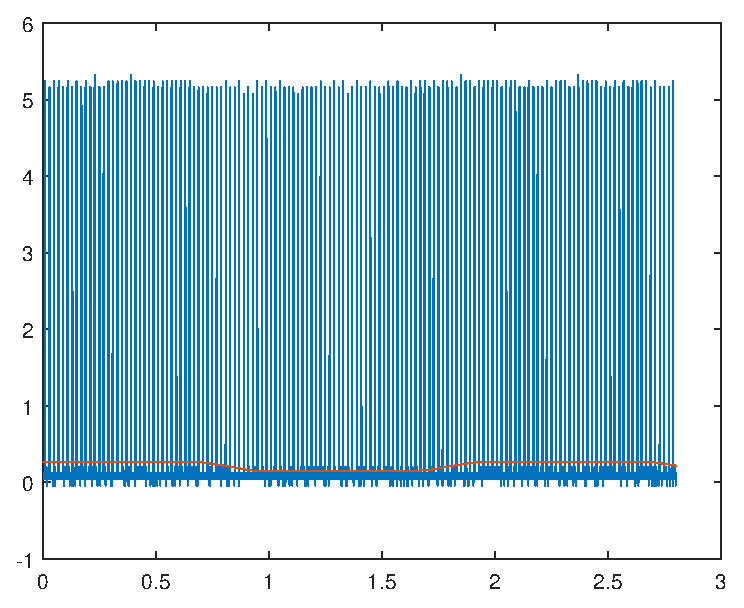
\includegraphics[width=\SchematicWidth]{\Images/Servos/time-domain-response.eps}
    \caption{Time domain servo response}
\end{figure}
\FloatBarrier

\paragraph{}
We can see on this image... nothing ! That's because the pulse length if near 0 compared to the whole
period. And even then, the servo response is quite slow, thus we need a long measure time !

To exploit this data, we used the Matlab "DutyCycle" function, that return the actual duty cycle of a signal.
This gave us results that where ok, but clearly perfectibles :

\begin{figure}[!hbt]
    \centering
    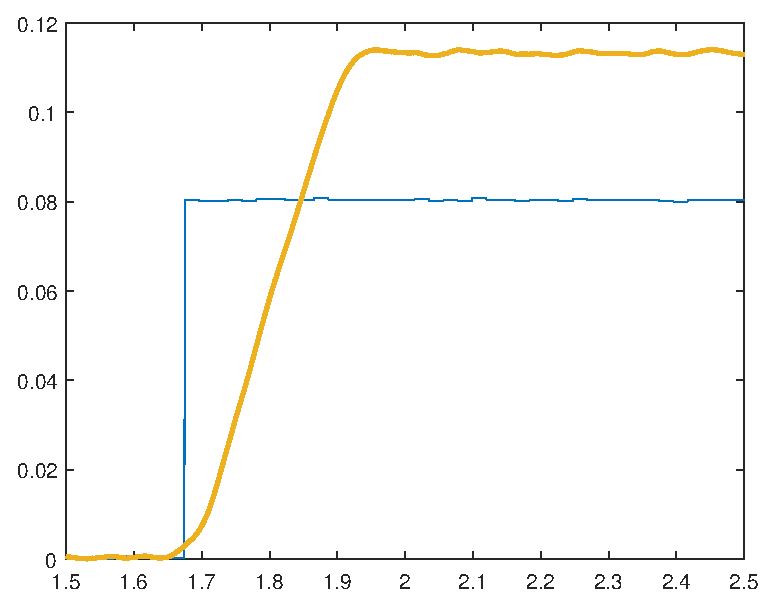
\includegraphics[width=\SchematicWidth]{\Images/Servos/Duty-Forced.eps}
    \caption{Time domain servo response, expressed in duty cycle}
\end{figure}
\FloatBarrier

\paragraph{}
Now, we have a command and a response that seem plausible, except one details : The servo seems to start
\textit{before} the command. That's typically the case for a non-causal systems, which can't be easily controlled,
if at all !
Luckily, in our case this is an issue from the code that draw theses graphes, rathers than the servo by itself.
We used a script that convert the raw measures to theses ones, but there was a bug, which cause this lag \footnote{
    To be precise, the DutyCycle function return a list of n elements, where n is the number of period. We then
    extended this list to match the original lenght. And since the DutyCycle return the value at the end of the
    period, there is $Te$ retard. Thus, a $\frac{1}{Te}$ period is now $\frac{n}{Te}$.
    Combine both, and you end up with a visually non-causal system.
}.

\paragraph{}
Anyway, theses measures weren't that good, they gave a first order approximation but didn't represented
correctly the signal. This was caused by multiple points :

\begin{itemize}
    \item Error on the signal generator : When working at this kind of low frequencies, the signal is quite imprecise.
    \item Too big amplitude on the command. This lead to results that are outisde the interresting range.
\end{itemize}

\paragraph{}
We addressed most of theses points on the second session of measure, where we used the final MCU to control the servos.
We thus got a precise (Up to $\pm 1 \si{\mu\second}$) pulses, and the definitive measure device (the integrated ADC)\footnote{
    Which was already characterized at this point, but, for clarity reasons is explicited in the next section
}.

We got theses measures :

\begin{figure}[!hbt]
    \centering
    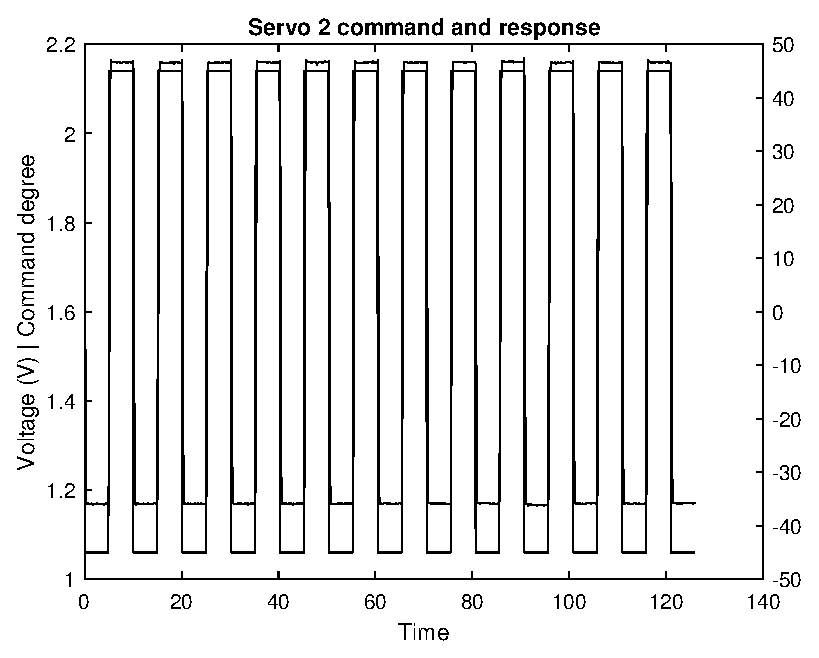
\includegraphics[width=\SchematicWidth]{\Images/Servos/reduced-square.eps}
    \caption{Time domain servo response, expressed in duty cycle}
\end{figure}
\begin{figure}[!hbt]
    \centering
    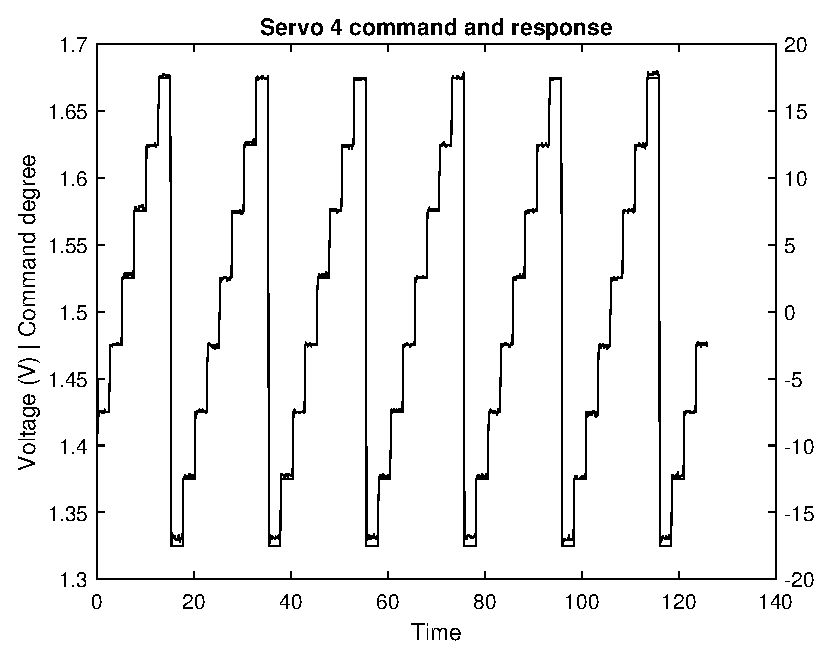
\includegraphics[width=\SchematicWidth]{\Images/Servos/ramp.eps}
    \caption{Time domain servo response, expressed in duty cycle}
\end{figure}
\FloatBarrier

\paragraph{}
Theses are way better than we got on the first session, because we addresses the issues.

Using the zoom functions, we can identify that in our case, the servos engines are responsing
as a very simple device : A first order one.

They goes into the required position in about $1 Te$, which is on our system arround
$120 \si{\milli\second}$ by achieving a linear transition.


\input{chapters/carac/part2/carac-wings.tex}
To conclude this part, let's talk about ADC deviations :

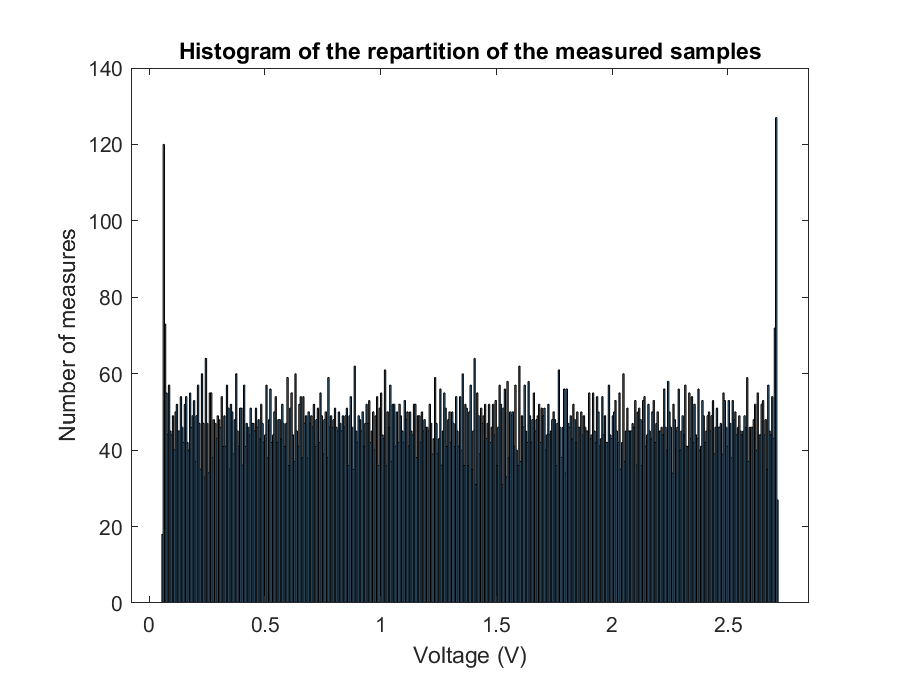
\includegraphics[width=\SchematicWidth]{images/ADC/ADC-DNL.eps}

\includegraphics[width=\SchematicWidth]{images/ADC/gain-error.eps}

\includegraphics[width=\SchematicWidth]{images/ADC/gain-compensated.eps}

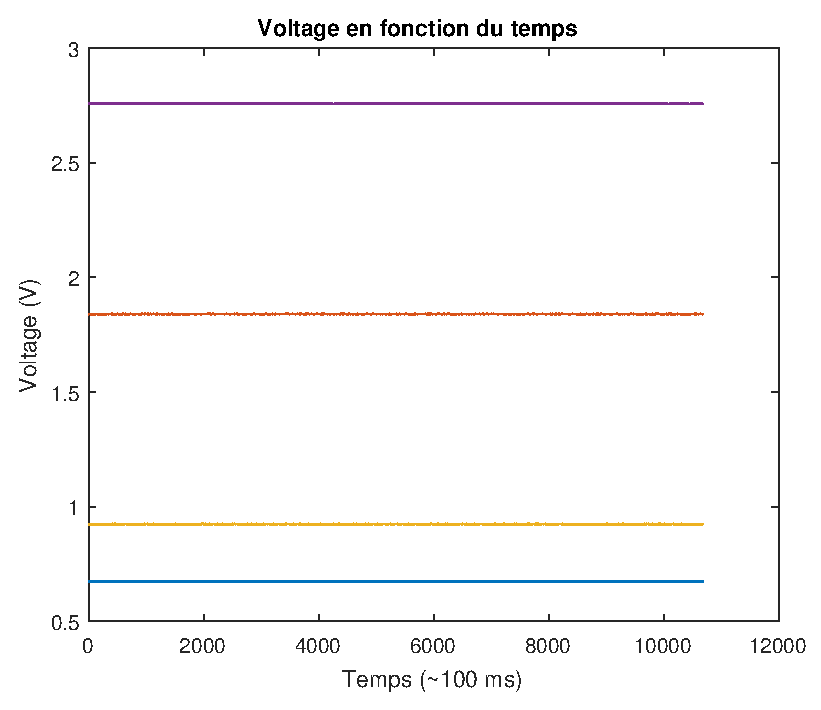
\includegraphics[width=\SchematicWidth]{images/ADC/time-deviation.eps}



\chapter{Mechanical design}
<<<<<<< HEAD
<<<<<<< HEAD
<<<<<<< HEAD
% This part is 100% on the annexes
=======
test 2
>>>>>>> cd3bfa6 (a test to test if the test was succesfully tested)
=======
=======
>>>>>>> d425107 (Merged main into mechanical)
test 2
=======
test

\section{Parachute mechanism}
Once launched, the rocket need an safe method to land back on earth. This mean
we need a parachute to be deployed once the rocket has got it's maximal
altitude.

But, this parachute need to be safely stored inside on rocket tube while
launching, to prevent any damages !

\subsection{Constraints}
To ensure a correct flight trajectory, we needed to place the parachute (which
is a quite heavy element) near the center of the rocket. This mean there is
some stuff above it.

This is an serious constraint, because we can't simply eject the tip of the
rocket to free the parachute, but we need to split the tube in half, while
ensuring structural rigidity of the tube while launching !

\subsection{Solutions}
To circumvent these constraints, we choose a locking mechanism, based on a
rotational lock.

There is two rings, one fixed to the tube, the other fixed to an axle in the
middle of the rocket. These two are bound together by four locks, for which a
rotating movement of the base will make them rotate, exposing a solid arm to
the outside.

These arms are going into slots in the second part of the tube, where they lock
themselves into, maintaining the both part of the tube together.

A final spring has been added in the inferior part of the tube to ensure the
top part will be ejected once the locks are removed.
>>>>>>> b6c5220 (Added a first part of the parachute, waiting for some schematics to explain more in details)
<<<<<<< HEAD
>>>>>>> a5be01c (Conflicts resolved)
=======
=======
% This part is 100% on the annexes
>>>>>>> 2b89c2e (Moved content to annexes)
>>>>>>> d425107 (Merged main into mechanical)


\chapter{Electronic design}
Let's talk about the electronic design

First, we're going to dig into the schematic we've done for the physical part
of controller. Thus, we're going to start with a global schematic part, where
we explain the organization of the pages, and then we'll dig a bit deeper into
the differents blocs.

The whole schematic is available at the end of this report, in the annexes
\ref{annex:schematic}.

\section{Power supplies}
Now, let's look a bit deeper on the power supplies, and how they're agenced.
\subsection{Power tree}
To represent the whole power supply organization, we drew a power tree, a schematic that
represent the power supplies.

\input{\Schematics/power-tree.tex}

On this schematic, there two main regulators, that are, in fact buck switching regulators.
But, there's three power sources :
\begin{itemize}
    \item   Vbus : The 5V that came from the USBC port when the board is plugged on a PC.
    \item   Vbatt : A battery that is charged to power up the MCU and all of the logic
          circuits.
    \item   Vbatt\_pyro : A battery that is charged to power up the servo engines and
          the thruster starter.
\end{itemize}.

As we can see in \ref{fig:power_tree}, we can configure the power supply as we need.
From the three sources, we're able to use a single one by tying both supply together.
And, we can even then supply the whole system with a single USB supply, but at a reduced
voltage. At the opposite, if needed, we can bypass the 5V buck system if we want to
power the servos and the engines with an higher voltage.

Selection is mainly done by jumper, which are big zero ohm resistors.

\subsection{DCDC buck design}
To design theses circuits, we used a reliable tool that may be found online, from
Texas Instruments : \cite{POWERDESIGNER}. We pass them the input conditions, such as
voltage, and the output wanted : voltage and current. The tool output then circuits
than can match the needs, and we need to select one, based on some settings :

\begin{itemize}
    \item   Space on board
    \item   Cost
    \item   switching frequency
\end{itemize}

Since we didn't require specific criterion on theses aspects, we choose the one that
was the easiest to solder. Then, we import the designed module into the schematic.

\section{Digital part}
For the last part, the digital one, we didn't needed a lot of reflexion. Most of
the design was already done on development kits, for example on the nRF5340DK
\cite{nRF5340DK}. Even for sensors, there is mostly the default
application example that need to be copied, and slightly adapted to our needs.

For example, the modifications we done :
\begin{itemize}[noitemsep]
    \item   Change configuration bootstrap to select one mode of the other.
    \item   Configure power supplies needed.
    \item   Configure I2C addresses.
\end{itemize}

\subsection{Pin attribution}
When a sensor need to be connected on the MCU, we attribute some pins. Since near
all of them are digitals, and then be swapped by software. Thus, we'll be using a
pin swapping functionnality in Altium to perform theses operations for us.

Thus, the pin attribution on the MCU is quite arbitrary since it will change by after.
\section{Analog conception}
Now, let's jump into the analog design we've done : There isn't many analog
circuitery on this board, and we only use it for two purposes :

\begin{itemize}[noitemsep]
    \item   Get the position feedback of the servos.
    \item   Monitor voltages on power rails.
\end{itemize}

For this part, we're measuring a DC voltage that moves between $~0.6
    \si{\volt}$ and $~2.4 \si{\volt}$ at a slow rate : It takes near $1
    \si{\second}$ to change from $0.6 \si{\volt}$ to $2.4 \si{\volt}$. For the
second part, we're measuring a static DC voltage, just to ensure the battery is
present and in it's operating range.

Since the voltages are already in our measurement range, and even more, in the
area where the integrated ADC is quite linear, we don't have a lot of signal
conditioning to do.

We've only designed a filter to remove any high frequency signals that may be
picked by the wires used. Thus, we designed a Sallen-Key active filter, with a
100 Hz cutoff frequency. This filter is absent from the power supply rail
measurements, since they are located on the PCB, and we can ensure the signal
integrity with a proper layout.

The circuit is the following one : \input{\Schematics/servo-filter.tex}

Using a SPICE simulator, we got this response :
\begin{figure}[!hbt]
    \centering
    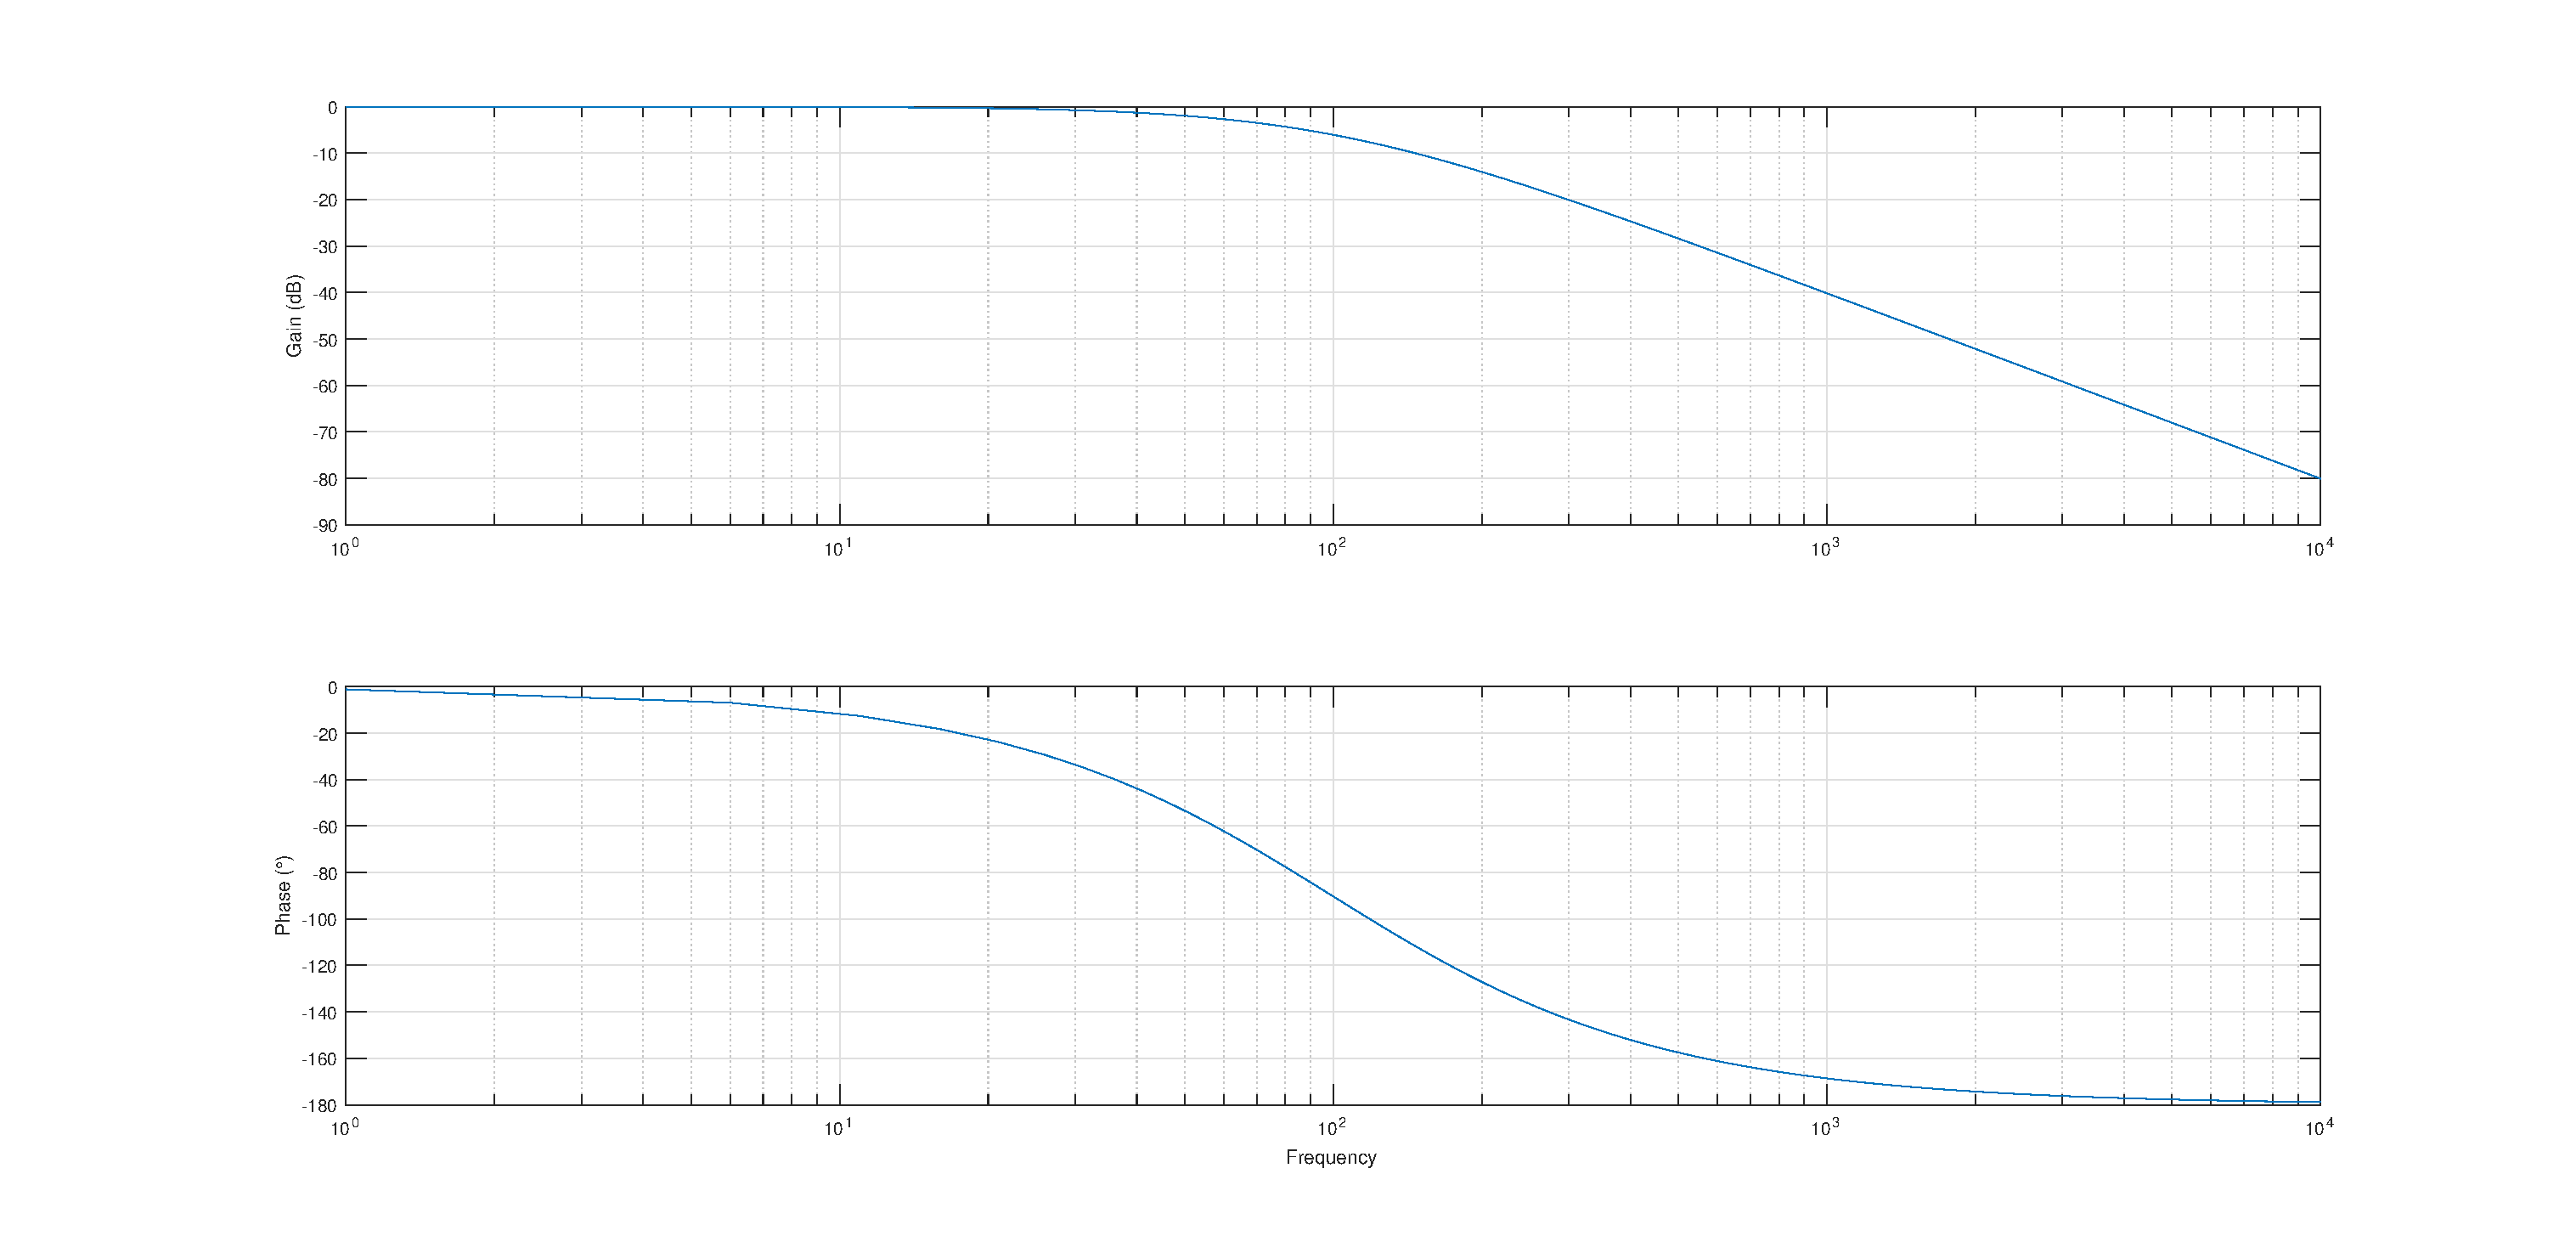
\includegraphics[width=\SchematicWidth]{\Images/Schematic/filter.eps}
    \caption{Bode plot of the filter response}
\end{figure}
\FloatBarrier

The response match our needs, which are quite simple : Remove the potential
harmfull noise, and fast variations that could occur.

The real circuit on the schematic is based on this one, but with optional
configurations jumpers to enable tuning the circuit on board.

This include :
\begin{itemize}[noitemsep]
    \item   An optionnal voltage divider at the input, to avoid putting the OpAmp in
          overvoltage.
    \item   Optionals jumpers to bypass the frontend directly to the ADC.
\end{itemize}
\section{Power section}
Now, let's look into the power section of the board. This is this section
responsible to power up the heaviest devices, which can't be powered from a
GPIO.

There's few devices on the board that require specific circuits to be driven :

\begin{itemize}[noitemsep]
    \item   The servomotors (ailerons and parachute).
    \item   The buzzer.
    \item   The engine starters.
\end{itemize}

Each of these elements go it's solution since they're requirements aren't the
same.

\subsection{Servomotors}
These devices are already an integrated solution, we don't directly drive the
servo. So, their power requirements are quite easy to fulfill : We feed them
with 5V, stable voltage.

We only used bulk capacitors near their connectors to ensure that a current
peak is handled it locally.

\subsection{Buzzer}
This second device is a different beast, since we drive it directly. This time,
we placed it directly on the supply, with an NMOS on the low side, to switch on
or off the current on it, and thus make sound, or not.

So, we needed an NMOS transistor to be choosen that can handle some current,
but more importantly : An NMOS that was compatible with our voltage level
available on the output of GPIOs\footnote{ The mosfet we choosed was working,
    the can be optimized : We didn't make sure that is was fully switched at our
    GPIO voltage level, and thats effectively the case : It fully switch at arround
    6V. Thus, the current is limited, which is fine for logic usages but not power
    ones. }.

\subsection{Engine starters}
For these last one, this is where our requirements are the highest : We need a
lot of current, around 2A per engine to start, at a quite high voltage (8-9V).

The power supply for this section is different than the remaining of the board,
for a simple reason : When the engine start, the supply is near the short
circuit. It's voltage will then drop, and it may place others components in
UVLO (UnderVoltage LockOut), where the device stop working.

Here we used ULN2803C drivers IC, made to handle a lot of current with
difficults loads (inductives, high voltage...). These are Darlington BJT
transistors pairs, with each channel done for 500mA. By using four channels in
parallel, we got our current requirements.

But, these IC require arround $ 1 \si{\milli\ampere}$ per input ! Here, that
wasn't an issue since these inputs are controlled by an AND gate
\ref{subsec:dis_logic}. This gate is able to provide more than enough current,
while preserving a low input current, perfect for an MCU or any GPIO.

\section{RF Antennas}
For this second section, we're going to explore some RF design steps that we done on the PCB,
to draw our antennas for the different modules.

This include a $1.55 \si{\giga\hertz}$ for the GPS signals, and a $2.4 \si{\giga\hertz}$
Bluetooth antenna.

For theses antenna, we've found a nice application note from TI \cite{InvertedF} that
show different examples of RF design for $2.4 \si{\giga\hertz}$  Antenna, and \cite{GNSS}
for the $1.55 \si{\giga\hertz}$ one. Since we don't really know how to properly design an
antenna from scratch, we copied theses design into our schematic and PCB while doing a
little bit of MATLAB simulation on the design to ensure the criterions will be matched.


\begin{figure}
\begin{minipage}[b]{0.24\textwidth}
  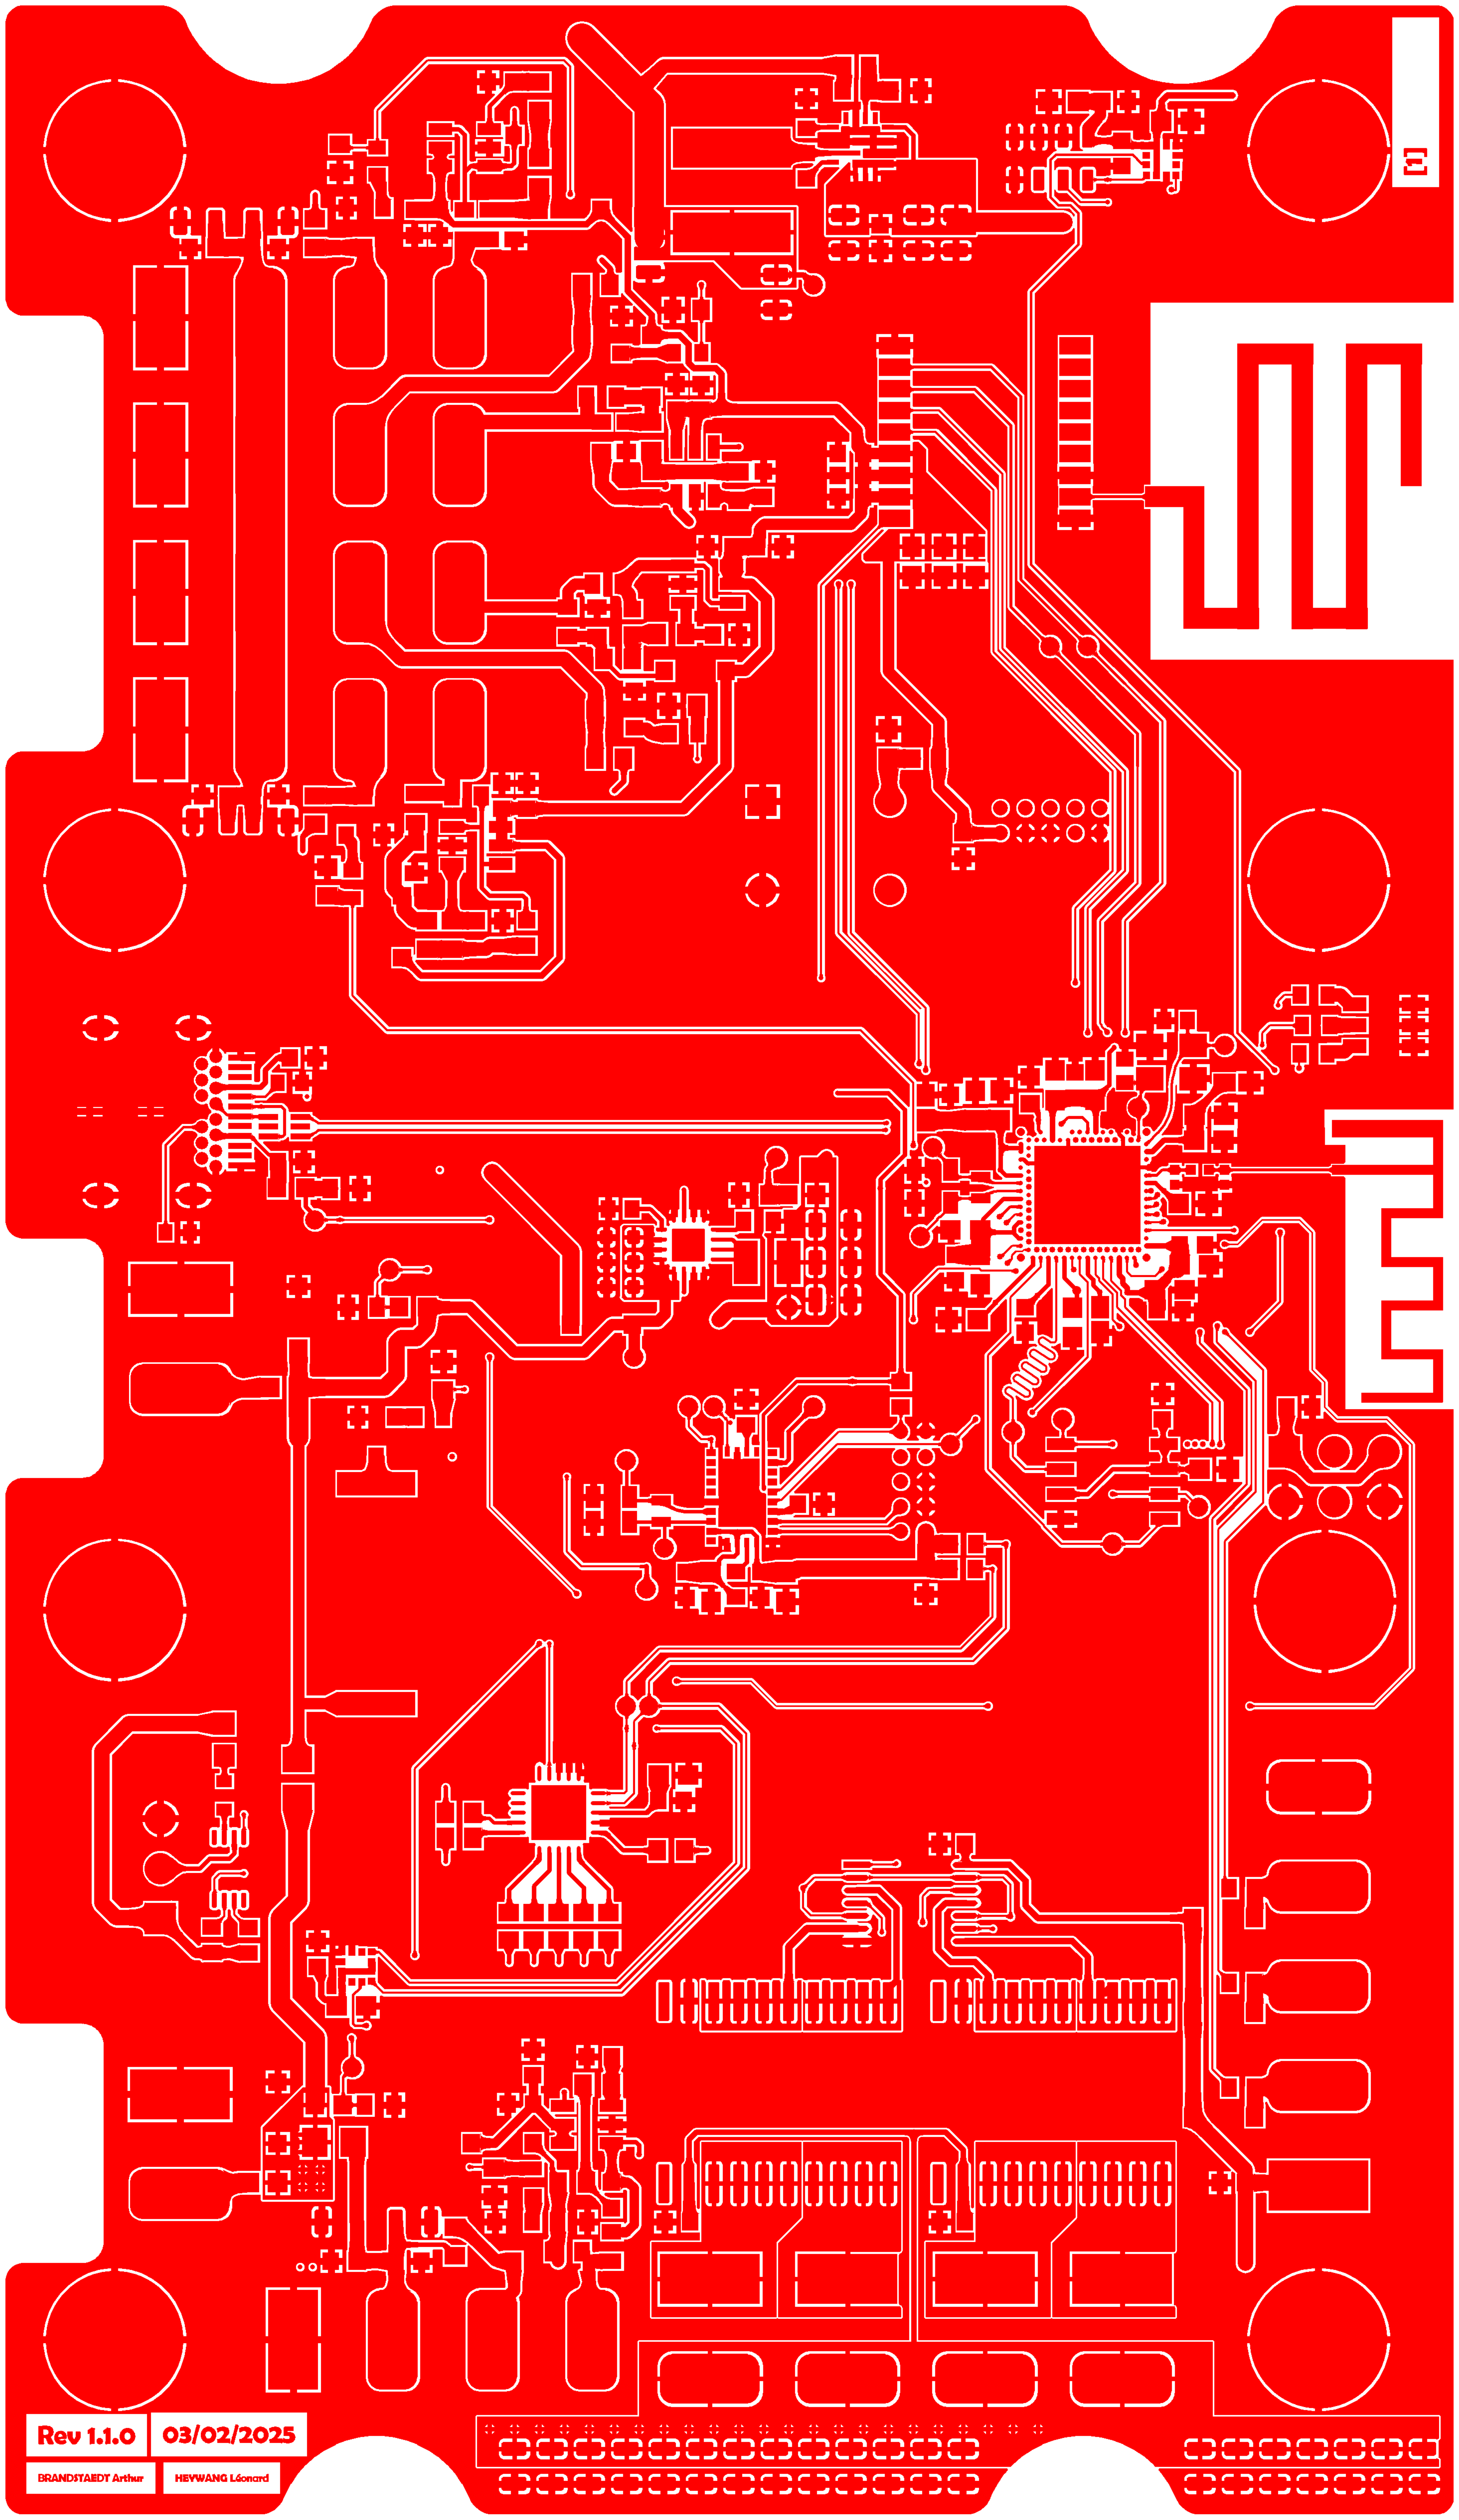
\includegraphics[width=\textwidth]{\Images/PCB/top.eps}
  \caption*{Copper layer (L1)}
\end{minipage}%
\hfill%
\begin{minipage}[b]{0.24\textwidth}
  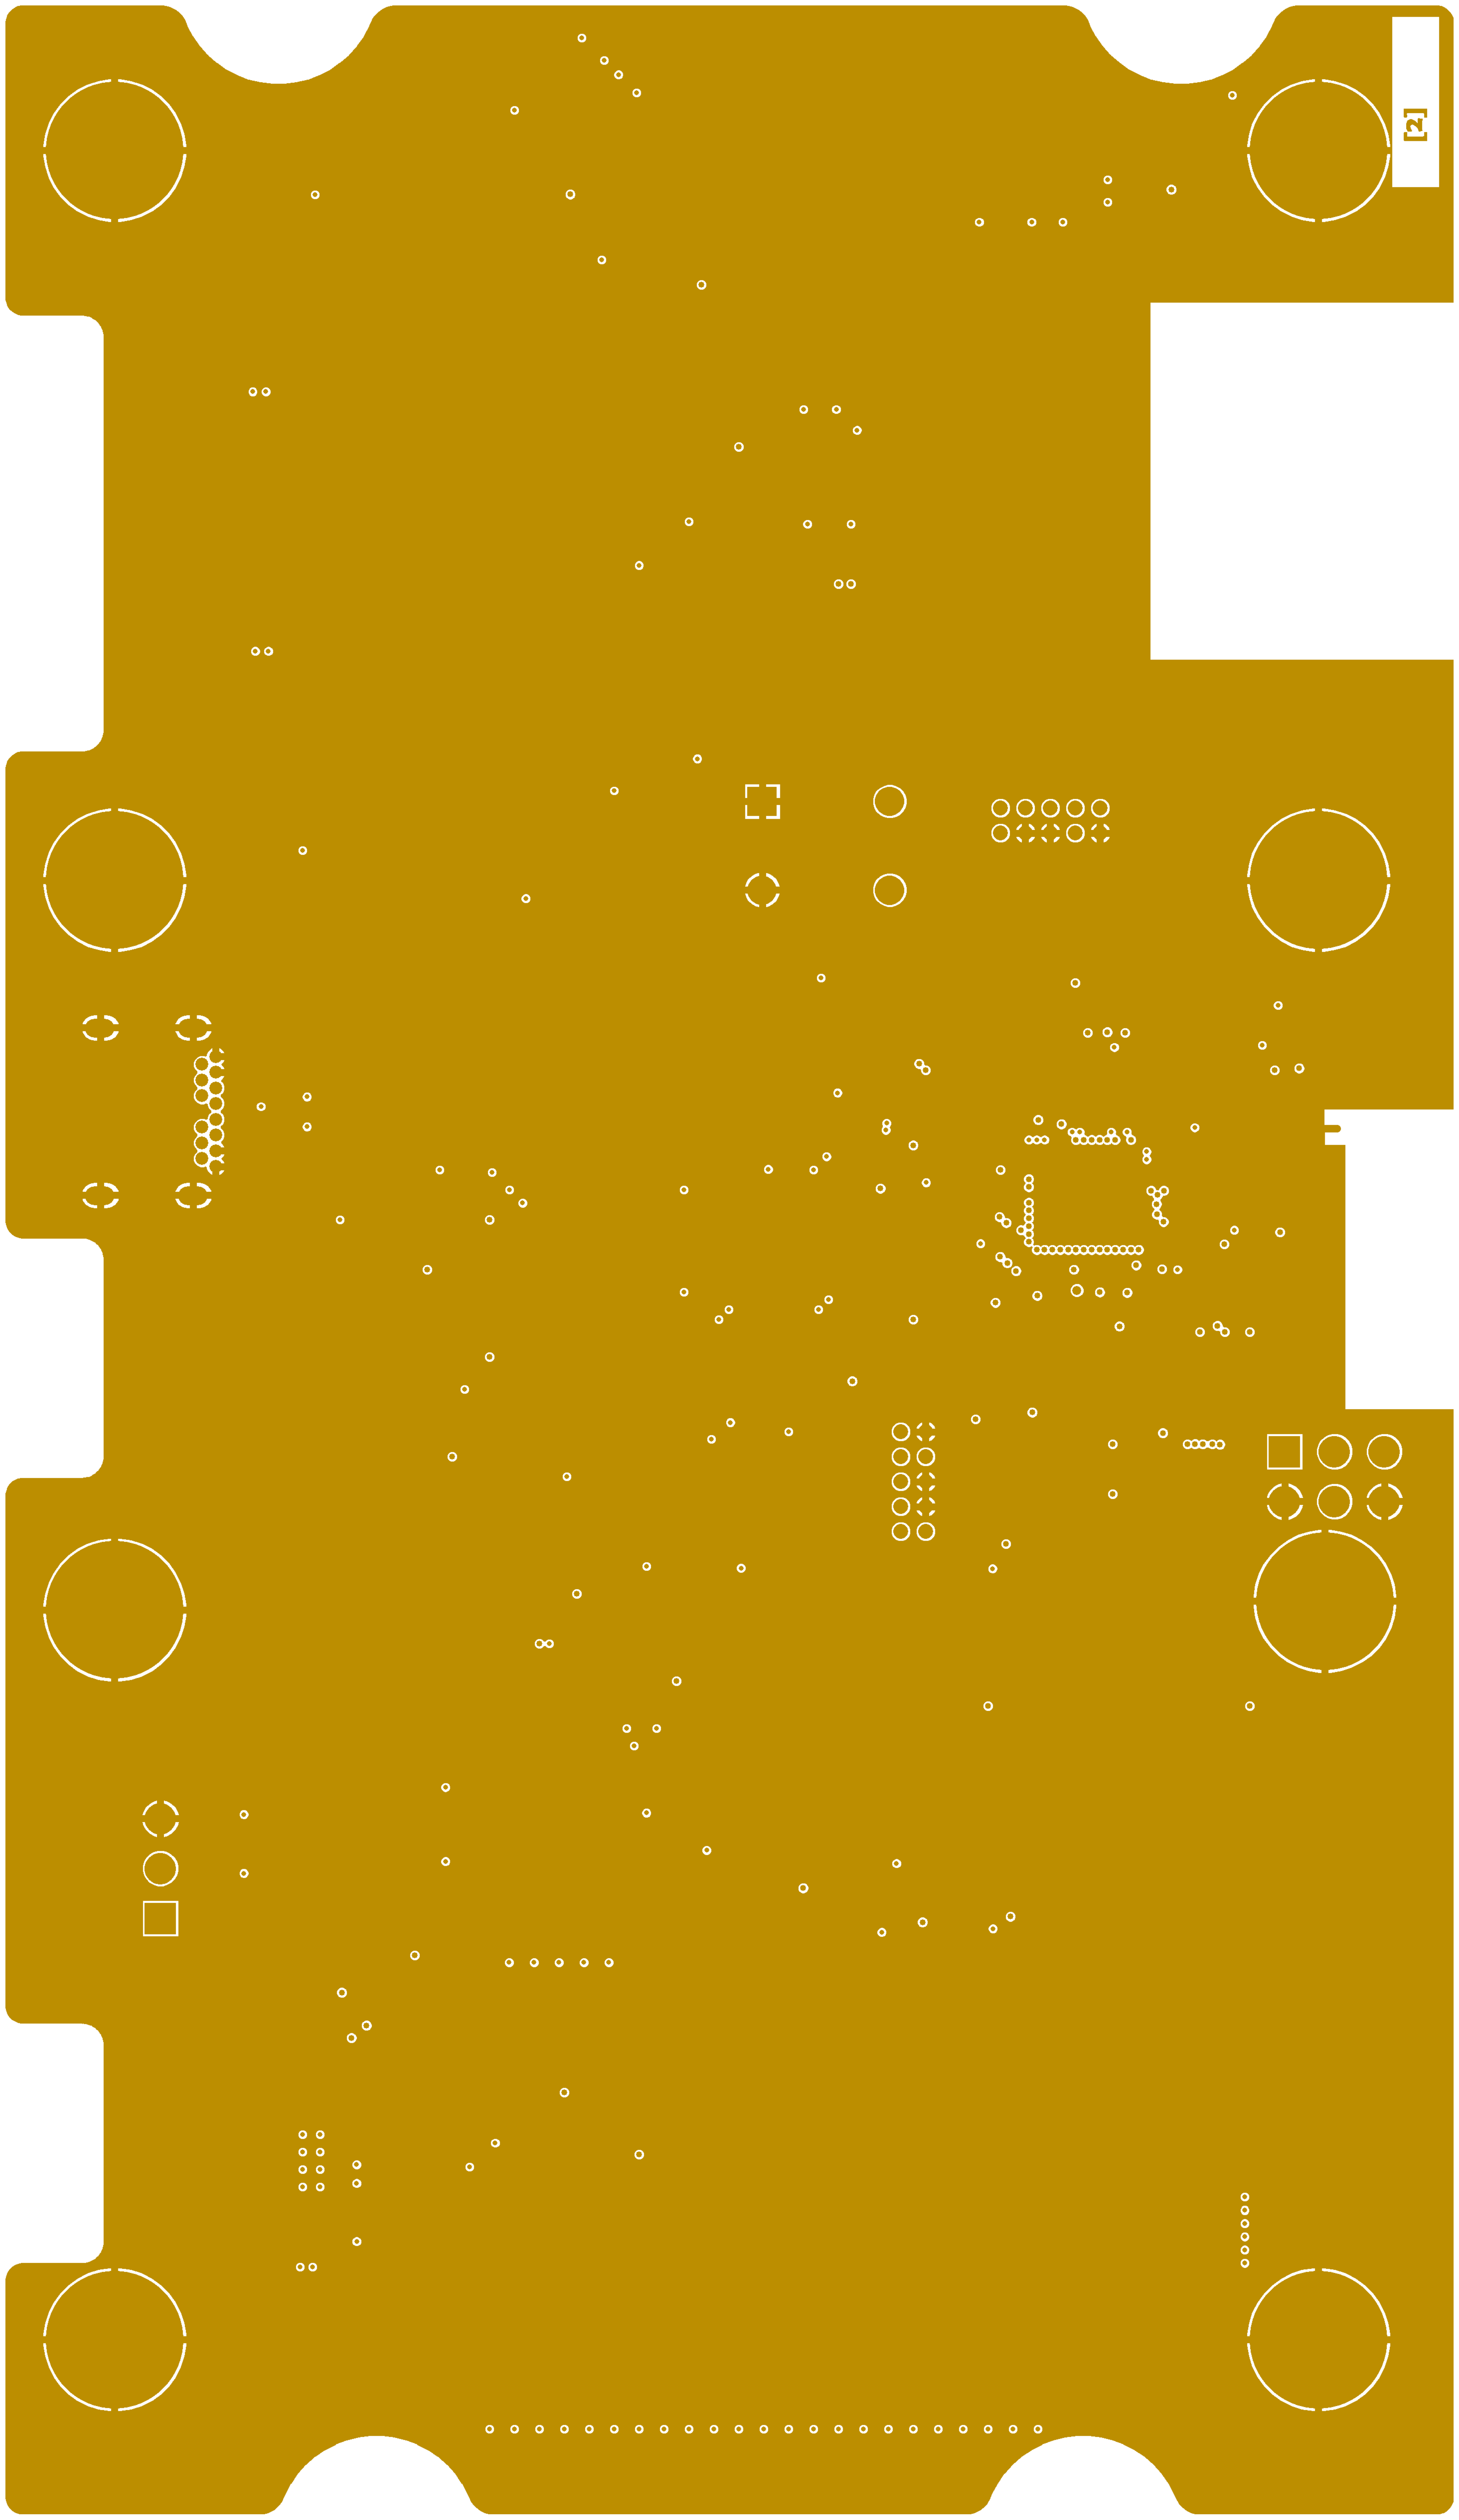
\includegraphics[width=\textwidth]{\Images/PCB/int1.eps}
  \caption*{Copper layer (L2)}
\end{minipage}%
\hfill%
\begin{minipage}[b]{0.24\textwidth}
  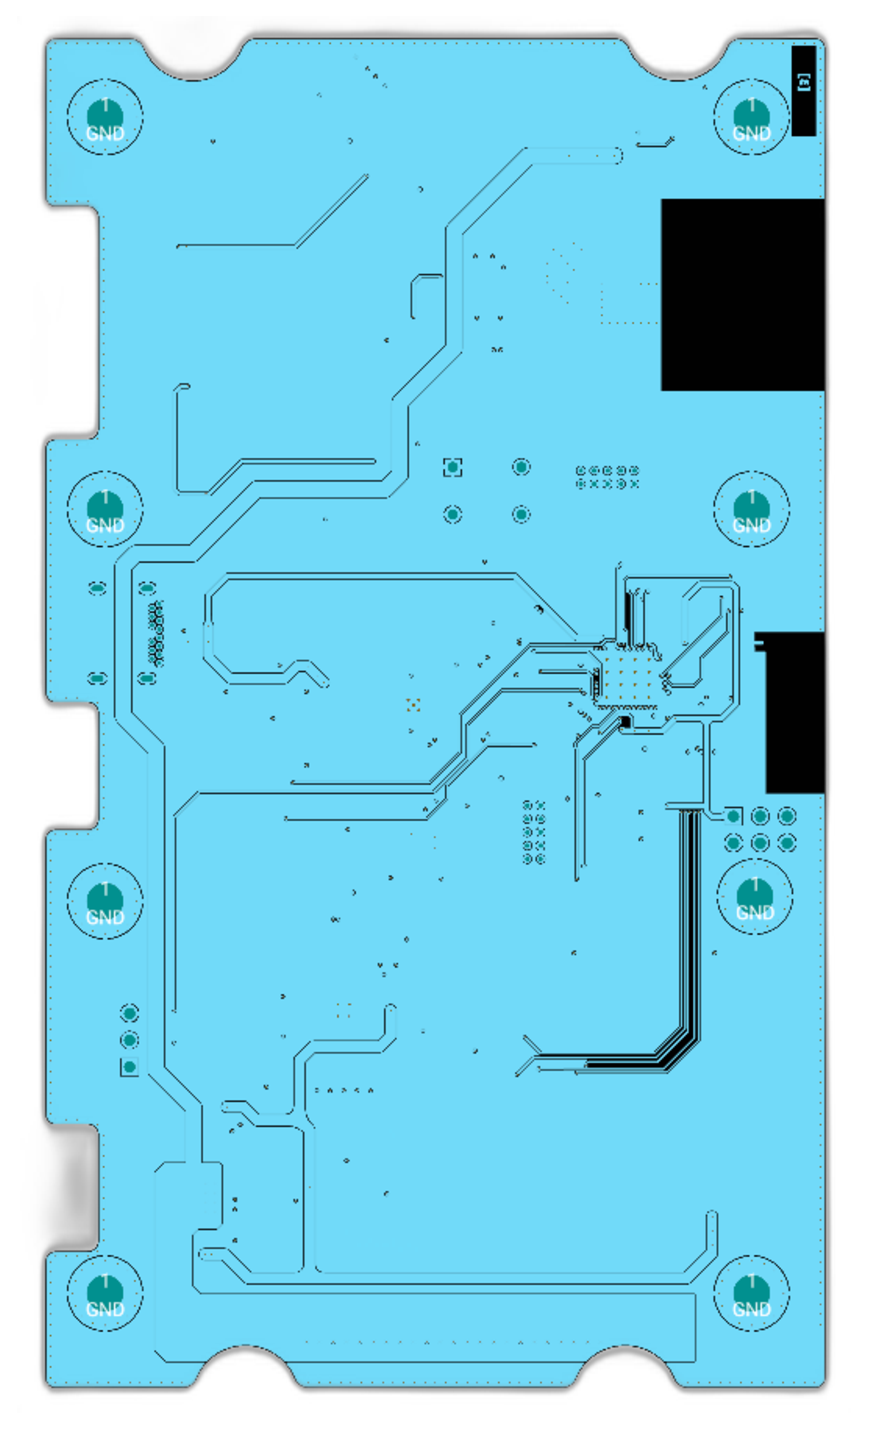
\includegraphics[width=\textwidth]{\Images/PCB/int2.eps}
  \caption*{Copper layer (L3)}
\end{minipage}%
\hfill%
\begin{minipage}[b]{0.24\textwidth}
  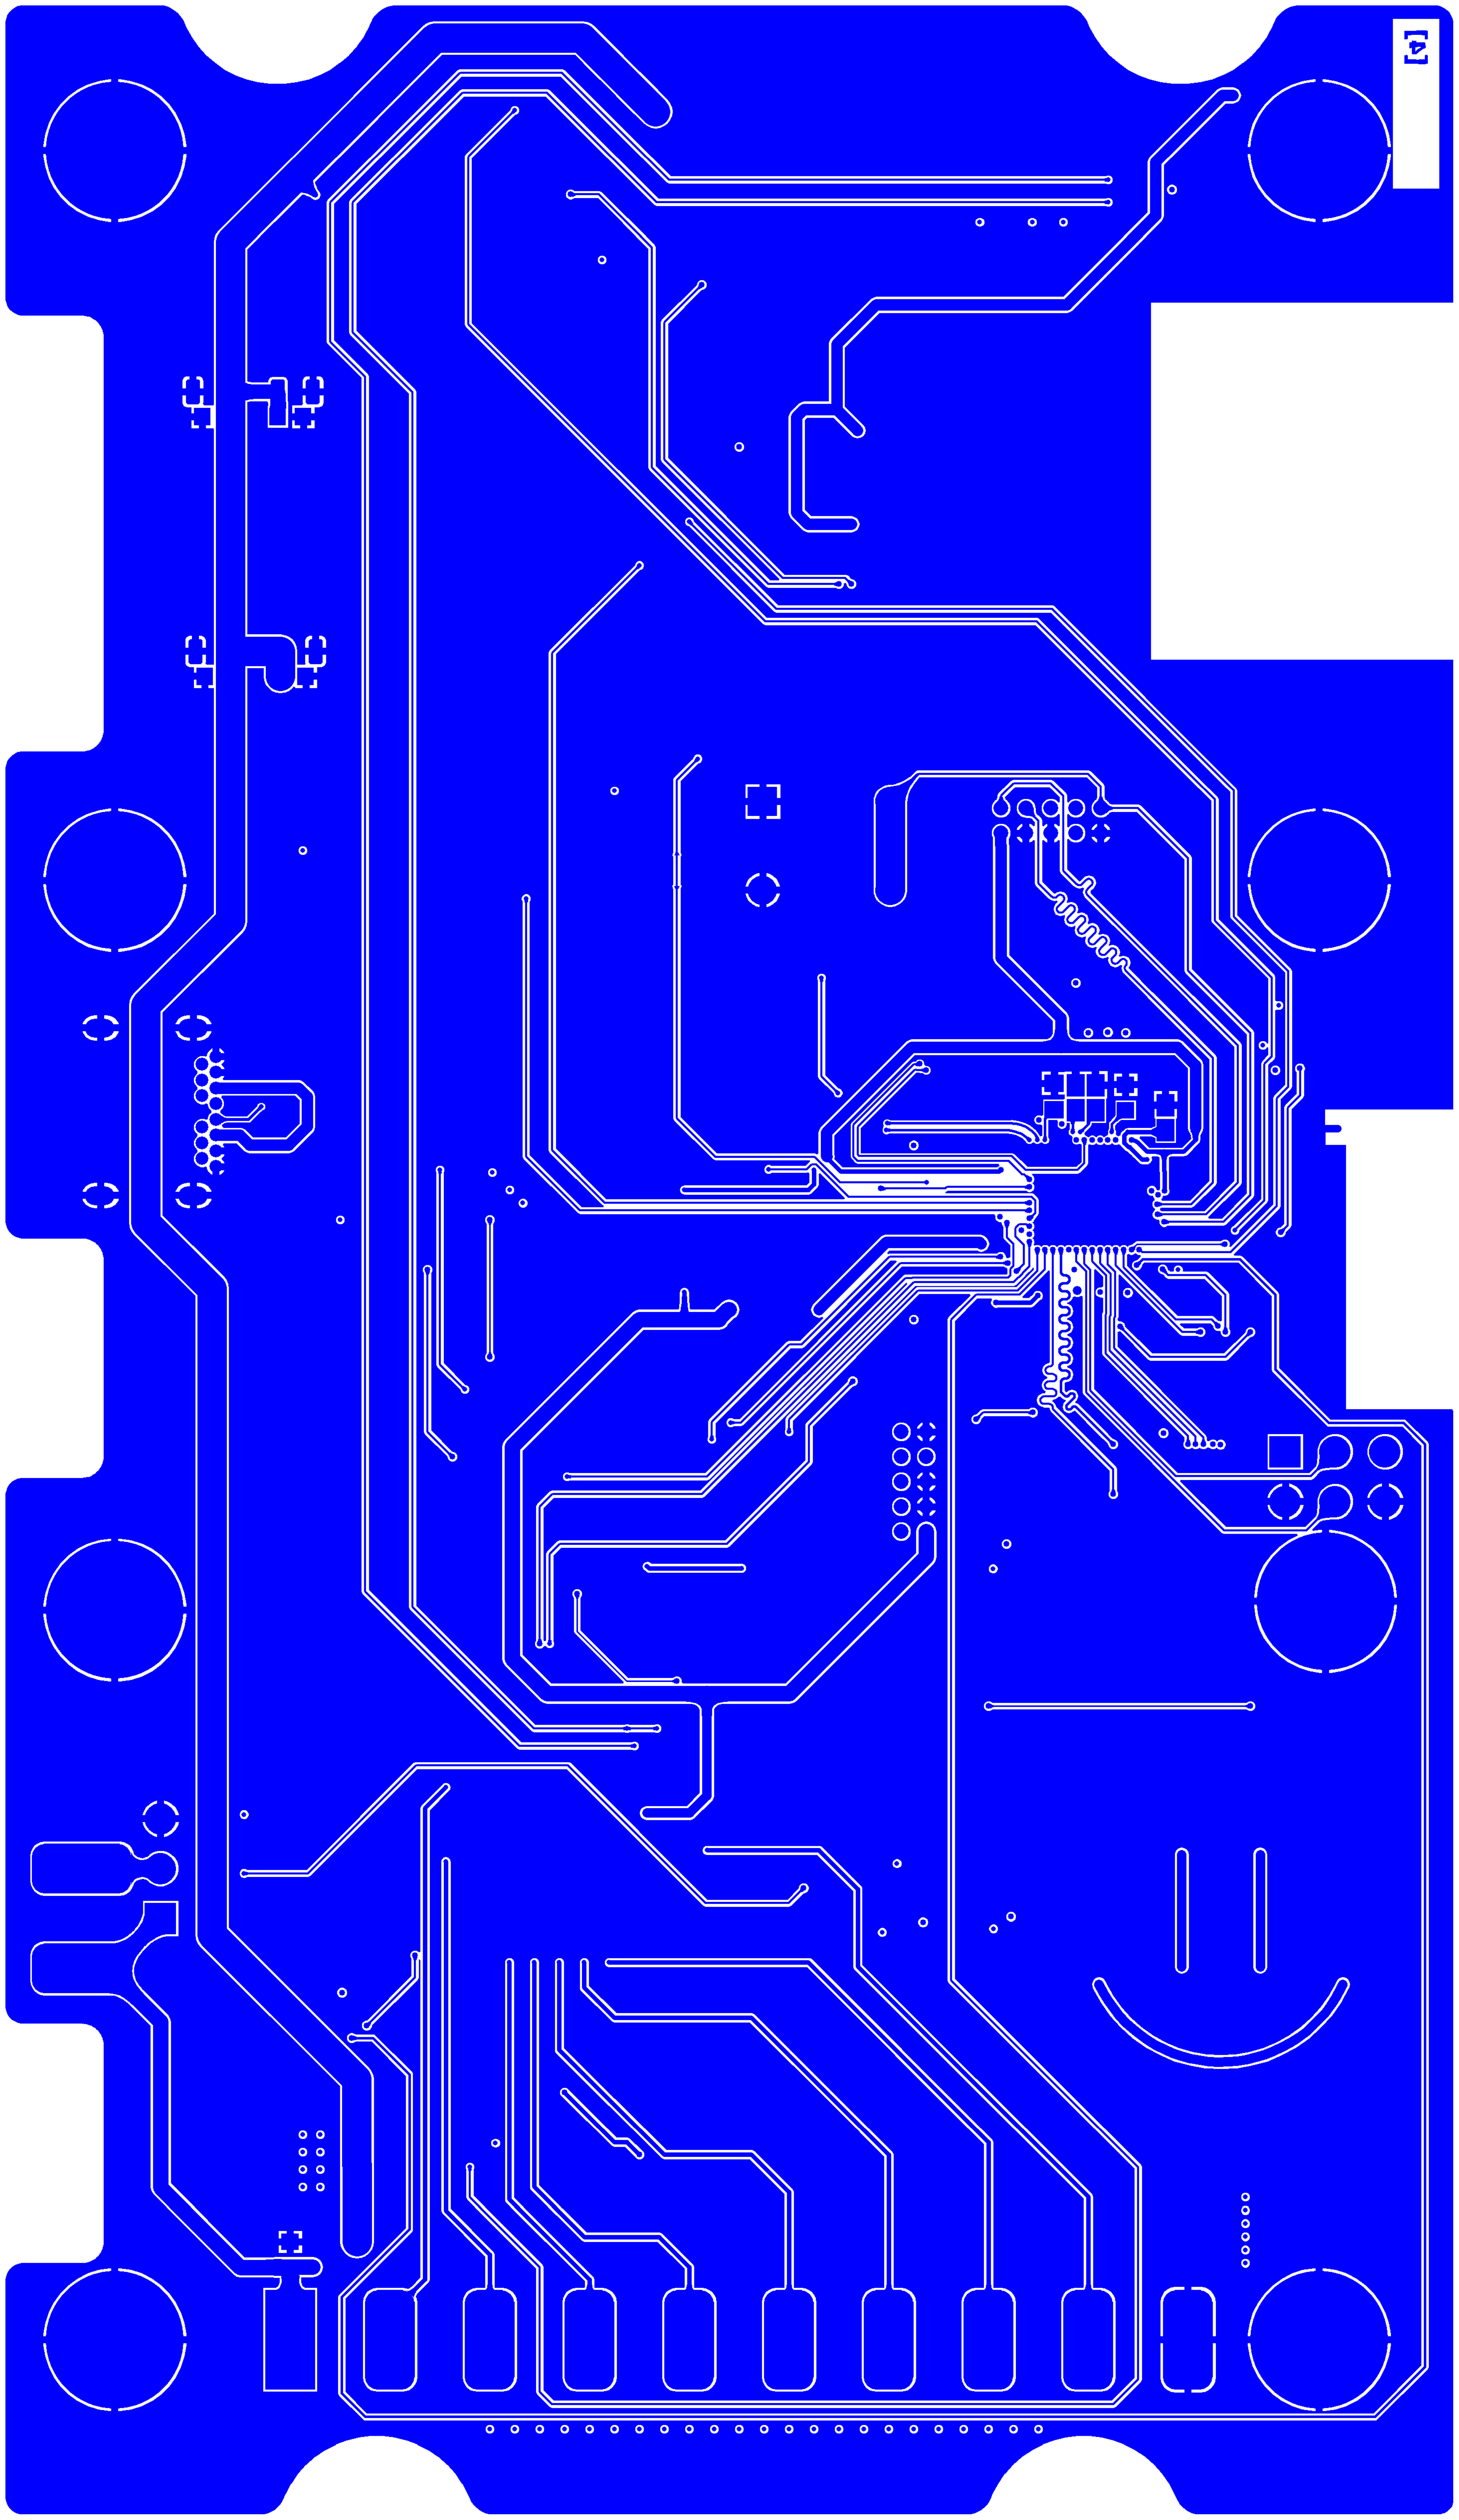
\includegraphics[width=\textwidth]{\Images/PCB/bot.eps}
  \caption*{Copper layer (L4)}
\end{minipage}
\end{figure}
\section{Soldering}\label{sec:assembly}
For the last part of the electronic chapter, we're going to talk about
assembly of the board.

The board use complex components, where the packages are BGA, aQFN...
All of the pitch are in the $0.5 \si{\mu\meter}$ range, thus, it's
evident that it won't be possible to solder it with an iron.

To solder theses components, we used a technic based on industrial
processes, which consists of different steps :

\begin{itemize}
    \item   Apply some solder pastes on the pads.
    \item   Place the ICs and passives on their spots.
    \item   Heat the whole board, to make the solder paste melt.
    \item   Let the board cool down.
\end{itemize}

Solder paste is a mix of tin and flux. It's used to create precision
soldering, since it's much easier to get the rigth volume of tin on a
point.

\subsection{Solder paste application}
First, we need to apply solder pastes. The smallest pads are round,
$200 \si{\mu\meter}$ in diameter, and $500 \si{\mu\meter}$ far from the
other.

It's then impossible to place solder paste by hand on this pads.

That's why we used a stencil, that we place over the board, and fix in
place with different tools. Then, we apply some paste on this stencil, and
we spread it on the board with something rigid enough.

This will fill the stencil holes with the right volume of paste, and, if
correctly placed, right over the pads. Once finished, we remove the stencil,
and there shall be right enough paste, we it needs. \footnote{
    Since the paste is about half flux, getting a bit of paste where it shouldn't
    isn't generally an issue. And, with surface tension of melted tin, it will
    generally flow to the contact without issues.
}

\subsection{Placing the SMT}
Once we're satisfied with the paste application, we can start to place components.

This step can be quite long, since it require a lot of application, and concentration.
Hopefully, there is some tools to make it easier, such as Altium assembly assistant,
which will prompt us which reference goes where, and in which orientation.

This make the placement much faster and right.

Once all components are placed, we inspect them. They need to be precisely placed
for all of them\footnote{
    When the board is hot enough, again, the surface tensions of the melted tin will
    tend to place the IC by themselves. Imprecisions can be corrected here, for a
    maximum of half the distance between two pads.
}. In our board, there is 286 of them !

\subsection{Heating}
For the final part, we need to heat the board. There is multiple solutions here,
we can do it on a specific furnace on the FabLab, or, with an hotplate at home.

We tried the second solution for the first board. This plate is going to heat to
$250 \si{\degree}$, heating the whole board in the same time. All of the paste will
melt in the "same" time, and thus all of the solder will be done in one time.

Once finished, we remove the board carrefully of the heating plate, and wait for it
to cool.

All of the process is in photo right below :

\begin{figure}[!hbt]
    \centering
    \begin{minipage}[c]{\SmallSchematicWidth}
        \centering
        \includegraphics[width=\textwidth]{\Images/assembly/assembly_STENCIL.eps}
        \caption*{Stencil placement}
    \end{minipage}%
    \hfill%
    \begin{minipage}[c]{\SmallSchematicWidth}
        \centering
        \includegraphics[width=\textwidth]{\Images/assembly/assembly_PASTE.eps}
        \caption*{Solder paste applied}
    \end{minipage}%
    \hfill%
    \begin{minipage}[c]{\SmallSchematicWidth}
        \centering
        \includegraphics[width=\textwidth]{\Images/assembly/assembly_SMT.eps}
        \caption*{PCB with the SMT placed}
    \end{minipage}%
    \hfill%
    \begin{minipage}[c]{\SmallSchematicWidth}
        \centering
        \includegraphics[width=\textwidth]{\Images/assembly/assembly_HOTPLATE.eps}
        \caption*{PCB on the heating surface}
    \end{minipage}
    \label{img:assembly}
    \caption{assembly process}
\end{figure}
\FloatBarrier

After that whole process, we need to add the few trough hole components, manually.
This is quite fast, since there is not a lot of them.

\chapter{Controller}
Let's talk about the controller design :

\input{\Src/control/part1/control-model.tex}
\input{\Src/control/part2/control-design.tex}
\input{\Src/control/part3/control-simu.tex}

\chapter{Programmation}
\paragraph{}
For this part, let's talk about a whole different beast : The software. This correspond to all of the code executed
on the microcontroller to command all of the actions done, from the control of the rocket trajectory to the log of
the temperature !

\paragraph{}
This is a very complex topic, that could be the subject of a whole report, so we're forced to reduce some part of it.
Nonetheless, we'll go trough all of the main subjects.
First, we'll talk about the configuration of the different functions by exploring the different devicetree files.
In a second time, we'll go trough the fundamentals of Zephyr RTOS, which was used to schedule main tasks and handle
the nasty memory stuff for ourselves.
Then, we'll start to ramp up into the different abstraction layers used, from the drivers to the threads.
To conlude this chapter, we're going to show the global software architecture we used over the project.

% Including all of the files
% Device trees
\section{Configuration using devicetrees}
Since we're using a microcontroller that is widely available, most of the work with
devicetrees has already been done by the manufacturer.

Thus, we don't need to care about memory, cpus, or other internals details of the
peripherals. We only edit properties that are related to our needs, which include
peripherals or other ICs.

All of the structure was automatically generated by a tool provided by the manufacturer,
that create an empty structure with everything needed to ensure the boot of the controller.

\paragraph{}
To make the structure cleaner, we've used a lot of overlays, because it's much easier
to debug and find the right property when needed.

\subsection{Main overlays}
Thus, the generated file has only a new line : the one needed to include the main overlay file.

This file look like this :

\inputminted[linenos, firstline=16, lastline=44]{devicetree}{\DeviceTree/topaze-pinctrl.dtsi}

This file is not a properly formed overlay, since it does indeed overlay nothing. But it make our
job easier by grouping all of the sub includes into a single file. Then, we can modify them for
debugging purposes.

We'll quickly move to another file that show a real overlay file, such as the PWM and I2C configuration.

\subsection{Peripherals overlays}
\subsubsection{PWM configuration}
Then, let's open a file like the PWM configuration to explore more in details what an overlay is.
For any overlay file, we used four main blocks\footnote{
    The number of block may vary depending on each architecture and software decision.
}, which are

\begin{itemize}
    \item Global peripheral configuration
    \item Pin configuration
    \item Advanced peripheral configuration
    \item Aliases
\end{itemize}

\paragraph{Global peripheral configuration} ~\\
First, we need to configure globally the peripheral.
\inputminted[linenos, firstline=17, lastline=21]{devicetree}{\DeviceTree/topaze-pwm-servo.dtsi}

Here, we're simply enabling the peripheral by setting it's status property to "okay". Then, we're
passing a reference to a pinctrl configuration, charged to define the pins. \footnote{
    The default name is mandatory, and is used by the RTOS to know what to do with theses pins once
    placed in low power modes. We're not using them here.
}

\paragraph{Pin configuration} ~\\
Then, right after, we're configuring the said pins. We pass a group of pins that are defined by a
macro, that return the pin number according input like the port, the pin, and some description.

\inputminted[linenos, firstline=24, lastline=33]{devicetree}{\DeviceTree/topaze-pwm-servo.dtsi}

As previously said, we're not using low power modes so we don't need them in our project. If they
were defined, we would see here two group of pins, one for each mode.

\paragraph{Advanced peripheral configuration} ~\\
Now, the main configuration part. That's where we configure most of the behavior of the PWM peripheral.

\paragraph{}
Before entering into the main details, we need to explain something : We created a node named "wings" here,
that is compatible with pwm-wings. This is a custom wrote specification for our needs that wait for
\begin{itemize}
    \item A pwm array with exactly four pwm channels
    \item A pwm period
    \item Some boundaries about the duty cycle (expressed in time domain)
\end{itemize}

\inputminted[linenos, firstline=52, lastline=66]{devicetree}{\DeviceTree/topaze-pwm-servo.dtsi}

Thus, we find here our custom node with our four servo-engines defined, and some settings.
Not all settings are used by the PWM peripheral to configure itself, but by the software that
import them as constants.\footnote{
    For example, min-pulse and max-pulse are used by the software to compute the required
    pulse for a defined angle.
}

\paragraph{Aliases} ~\\
Then, to conclude on this file, we define some aliases. Theses enabled the fetching of a node by quoting
it's name rather than it's location.

\inputminted[linenos, firstline=69, lastline=74]{devicetree}{\DeviceTree/topaze-pwm-servo.dtsi}

\subsubsection{I2C configuration}
Then, in the same manner we configured the I2C \footnote{
    And a lot of other peripherals !
}. The file expose the same structure, as any overlay in the project.

\inputminted[linenos, firstline=36, lastline=61]{devicetree}{\DeviceTree/topaze-I2C.dtsi}

The main difference with the previous file is the presence of multiple nodes here, once for each I2C sensor.
Each device can has some properties, such a compatible, status and reg properties. The last one, reg,
correspond to it's address on the bus ! Thus, we don't care about such details on the software, we communicate
with a sensor, not a peripheral on some address.

\subsection{Final words}
To conclude this part, let's resume a bit the devicetree files. Theses are used for hardware related configuration,
and expose some options that may be used to directly configure the registers of an IC, or be exposed to a C or C++
as constants for more advanced usage. They're used by the underlying OS on the MCU while the pre-kernel boot.

Theses files are complex to write, but can be used to configure precisely the differents hardware while reducing
user errors.


% Drivers
\input{\Src/prog/HAL/prog-drivers.tex}
\section{Device drivers}
Next, let's ramp a bit higher in the software structure. Now that we have drivers for
most simple peripherals, we'll need drivers for devices, to handle all of the specific
protocols for us.

Thus, when we need to read a temperature, we don't want to write to a register, wait for
some time, and then read. We want to call a function that return us the temperature.

That's the exact job for a device-driver.
It format requests, use the peripherals drivers to handle the IO, and then make some
calculations to return us a precise value in any cases.

These kind of drivers can be sourced from the manufacturer, but some need to be wrote by
hand. Others need to be modified to be compatible with our software decisions. Some
other only provide standard libraries for the drivers, and let the user develop they're
own drivers.

\subsection{Manufacturer sourced drivers}
In the first case, which is the preferred option, the work needed is generally small.
For example, the driver for the IMU was entirely wrote by Bosch, which require us to
write only the communication functions !

This look like :
\inputminted[linenos, firstline=19471, lastline=19515]{cpp}{\Code/drivers/bno055/bno055.cpp}

And, that's done for the driver !

\subsection{Libraries based drivers}
In this second case, the manufacturer only provided some standard libraries to be used.
An lot of work was needed to ensure this driver is correctly working.

In the previous code section, the manufacturer provided a write and read functions to be
called. It only required us to fill them.

\inputminted[linenos, firstline=292, lastline=330]{cpp}{\Code/drivers/teseo/teseo.cpp}

Hopefully, manufacturer provided us some functions to check if a command was well
formed, to match the checksum, as well as some parsers to identify the different
elements.

This save us a lot of time compared to writting the full driver.

In this example of code, the manufacturer provided the GNSS\_PARSER\_CheckSanity functions
and other return values codes.

We only needed to implement the IO.

\subsection{Hand written drivers}
Even if theses drivers are quite complex to write, they're generally reserved to much
smaller chips, which make the develop quite straightforward.
For example, the only driver we needed to develop like that was for the temperature
sensor.

\inputminted[linenos, firstline=119, lastline=158]{cpp}{\Code/drivers/ms5611/MS5611.cpp}

This driver include all of the calculations needed for temperature corrections
needed to match the precision. Theses are indeed affected by temperature,
or just measure range. The sensor isn't linear at all over the plage, but per
segments.

Here, all of the code was hand written because nothing, except documentation was provided.


\subsection{Final words}
To conclude this part on drivers, we can resume them as a fundamental brick of the software,
that handle all of the device specific requirements.
This part part is generally where the errors are, because they're difficult to test entirely.

% Gloval architecute
\section{Architecture}
For this final section on the software architecture, let's talk about the top of the pyramid.
Now, we have a fully configured chip, devices drivers, and an RTOS ready to handle task.

We just need to create the differents elements to communicate, and connect them together.

Theses elements are :

\begin{itemize}[noitemsep]
    \item   A safety task, charged to ensure the authorisation to start.
    \item   A measurement task, charged to acquire all of the sensor data on the rocket.
    \item   A logger task, charged to log events and measure for a further usage.
    \item   A controller task, charged to compute and apply the commands for the different actuators.
\end{itemize}

Each of theses task communicate which each other trough three ways :

\begin{itemize}[noitemsep]
    \item   Some FIFO, from one task to the other. Used for data exchanges such as measurement data mostly.
    \item   A global status register, where each bits has it's own meaning.
    \item   A global messaging systems, where each thread can sen a global message to each others. Used to indicate errors codes.
\end{itemize}

Each of theses tasks has some input data, that came from the measurement task, and some outputs that are
reserved peripherals or part of peripherals. The software is done to ensure a single task will access to the SPI peripheral.

Graphically, this may look like :

\begin{figure}[!hbt]
    \centering
    \resizebox{\SchematicWidth}{!}{%
        \begin{circuitikz}
            \tikzstyle{every node}=[font=\normalsize]
            \draw [ fill={rgb,255:red,158; green,148; blue,213} ] (1.25,8.5) rectangle  node {\normalsize Measurement task} (7.5,3.5);
            \draw [ fill={rgb,255:red,236; green,195; blue,195} ] (11.25,14.75) rectangle  node {\normalsize Safety task} (17.5,12.25);
            \draw [ fill={rgb,255:red,236; green,195; blue,195} ] (11.25,7.25) rectangle  node {\normalsize Controller task} (17.5,4.75);
            \draw [ fill={rgb,255:red,236; green,195; blue,195} ] (11.25,-0.25) rectangle  node {\normalsize Logger task} (17.5,-2.75);
            \draw [->, >=Stealth] (7.5,6) -- (11.25,6);
            \draw [->, >=Stealth] (10,-1.5) -- (11.25,-1.5);
            \draw [->, >=Stealth] (10,13.5) -- (11.25,13.5);
            \draw [short] (10,-1.5) -- (10,4.75);
            \draw [short] (7.5,4.75) -- (10,4.75);
            \draw [short] (10,13.5) -- (10,7.25);
            \draw [short] (7.5,7.25) -- (10,7.25);
            \draw [ fill={rgb,255:red,162; green,199; blue,179} ] (20,-0.25) rectangle  node {\normalsize SPI EEPROM} (26.25,-2.75);
            \draw [ fill={rgb,255:red,162; green,199; blue,179} ] (20,11) rectangle  node {\normalsize Wings control} (26.25,8.5);
            \draw [ fill={rgb,255:red,162; green,199; blue,179} ] (20,14.75) rectangle  node {\normalsize Status LED} (26.25,12.25);
            \draw [ fill={rgb,255:red,162; green,199; blue,179} ] (20,7.25) rectangle  node {\normalsize Wings control} (26.25,4.75);
            \draw [->, >=Stealth] (17.5,6) -- (20,6);
            \draw [->, >=Stealth] (17.5,13.5) -- (20,13.5);
            \draw [->, >=Stealth] (17.5,-1.5) -- (20,-1.5);
            \draw [->, >=Stealth] (18.75,9.25) -- (20,9.25);
            \draw [->, >=Stealth] (18.75,10.25) -- (20,10.25);
            \draw [short] (18.75,9.25) -- (18.75,6)node[pos=0.5, fill=white]{Command};
            \draw [short] (18.75,10.25) -- (18.75,13.5)node[pos=0.5, fill=white]{Enable};
        \end{circuitikz}
    }%
    \caption{Task organizations}\label{tkz:tasks}
\end{figure}
\FloatBarrier

This architecture has been choose to ensure a sepration between tasks, and thus some security. If something went wrong on the logger
task, the controller would not be affected, because they're independant.




% Set page number in uppercase roman (I, II, III)
\chapter*{Conclusion}
\pagenumbering{Roman}

\addcontentsline{toc}{chapter}{Conclusion}
\paragraph{}
This is the point at which we were able to achieve this in approximately
eight months. The project is extremely dense, encompassing a wide range
of disciplines, including electronics design, flow mechanics, conventional
mechanics and even more.

\paragraph{}
This project was an eye-opening experience considering the complexity
and the need to comprehend so many different phenomena.
To sum up our work order in terms of parts, we first designed our rocket
in a gross simulation, we then designed in parallel the rocket in 3D and
did the electronics part. This last part was very time consuming to choose
every component and to build and encode the ecosystem of peripherals around
our MCU.

\paragraph{}
Once our first 3D rocket design was finished, we defined our constants like
the inertia matrix needed for our simulation. Once this was finished, we
developed our simulation using Simulink and a lot of help from Mr Schwartz,
Mr.Laroche and Mr.Nageotte who guided us and showed us what work we could
take inspiration from because this simulation isn't entirely self-made.
Every equation and every link between real-life and numerical equation was
made thanks to the work of those cited in the bibliography.

\paragraph{}
We are now at this point where we calculated and simulated our rocket to
start making it and where we have a mostly working PCB. We now need to print
and assemble our rocket and finish coding our MCU.
To sum up, this project was a "multidisciplinary nightmare" to call it badly
because we had to learn a lot of things which interacted between each other
as well as how to simulate it accurately to determine many parameters of
our rocket. The theory is done, we just need to finish the practice.

\paragraph{}
We would also like to thank all the teachers and educational staff for
their invaluable help throughout the project.

\vspace{5cm}
\begin{minipage}[c]{1\textwidth}
    \raggedleft
    We would like to express our gratitude to all those who have taken the time to read this document. \\
    BRANDSTAEDT Arthur \\
    HEYWANG Léonard
\end{minipage}


\chapter*{Bibliography}
\addcontentsline{toc}{chapter}{Bibliography}
\printbibliography

\newpage
\appendix

\end{document}
